% Generated by eval/scripts/write_mechanistic_latex_assets.py from the

% mechanistic-results artifacts. Figure and table macros for the exploratory

% mechanistic chapter; invoke e.g. \MechDirectionSimilarityFigure.

\newcommand{\MechDirectionConstructionFigure}{%
\begin{figure}[htbp]
\centering
\begin{tikzpicture}[x=1.15cm,y=1.0cm,>=Stealth]
\fill[red!65] (-2.75,-0.35) circle (1.7pt);
\fill[red!65] (-2.35,0.28) circle (1.7pt);
\fill[red!65] (-1.75,-0.42) circle (1.7pt);
\fill[red!65] (-1.45,0.20) circle (1.7pt);
\fill[blue!70] (1.25,0.10) circle (1.7pt);
\fill[blue!70] (1.65,0.72) circle (1.7pt);
\fill[blue!70] (2.20,0.05) circle (1.7pt);
\fill[blue!70] (2.55,0.70) circle (1.7pt);
\fill[red!85!black] (-2.05,-0.07) circle (2.5pt) node[below=3pt,font=\scriptsize] {$\mu_{\mathrm{unsafe}}$};
\fill[blue!85!black] (1.91,0.39) circle (2.5pt) node[below=3pt,font=\scriptsize] {$\mu_{\mathrm{refusal}}$};
\draw[->,very thick,violet!85!black] (-2.05,-0.07) -- (1.91,0.39) node[midway,above=6pt,font=\scriptsize] {$\hat r=(\mu_{\mathrm{refusal}}-\mu_{\mathrm{unsafe}})/\lVert\mu_{\mathrm{refusal}}-\mu_{\mathrm{unsafe}}\rVert$};
\fill[black] (-0.15,1.20) circle (1.8pt) node[above,font=\scriptsize] {prompt activation $h$};
\draw[densely dashed,black!60] (-0.15,1.20) -- (-0.04,0.17);
\fill[black!70] (-0.04,0.17) circle (1.5pt);
\node[font=\scriptsize,align=left,anchor=west] at (2.85,-0.65) {$z=(h-m)^\top\hat r$\\$m=(\mu_{\mathrm{refusal}}+\mu_{\mathrm{unsafe}})/2$};
\node[font=\tiny,text=red!75!black] at (-2.05,-0.85) {unsafe outcomes};
\node[font=\tiny,text=blue!75!black] at (1.91,-0.85) {refused outcomes};
\end{tikzpicture}
\caption[Construction of the refusal-outcome direction]{Construction of the refusal-outcome direction. The vector is the normalized difference between the mean final-prompt-token activation for refused and unsafe outcomes; a prompt is summarized by its signed projection $z$ onto that axis. This is a schematic of the computation, not a two-dimensional embedding of the observed 4,096-dimensional activations.}
\label{fig:mechanistic-direction-construction}
\fonte{Author, following \textcite{arditiRefusalLanguageModels2024}.}
\end{figure}
}

\newcommand{\MechDirectionSimilarityFigure}{%
\begin{figure}[htbp]
\centering
\scriptsize
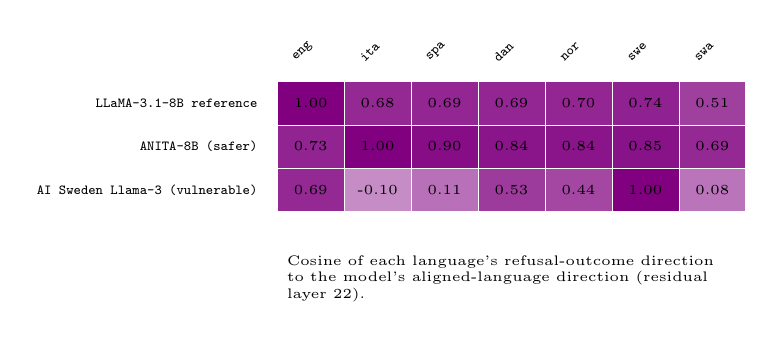
\begin{tikzpicture}[x=0.85cm,y=0.55cm]
\node[rotate=45,anchor=west,font=\tiny] at (0.16,0.35) {\texttt{eng}};
\node[rotate=45,anchor=west,font=\tiny] at (1.16,0.35) {\texttt{ita}};
\node[rotate=45,anchor=west,font=\tiny] at (2.16,0.35) {\texttt{spa}};
\node[rotate=45,anchor=west,font=\tiny] at (3.16,0.35) {\texttt{dan}};
\node[rotate=45,anchor=west,font=\tiny] at (4.16,0.35) {\texttt{nor}};
\node[rotate=45,anchor=west,font=\tiny] at (5.16,0.35) {\texttt{swe}};
\node[rotate=45,anchor=west,font=\tiny] at (6.16,0.35) {\texttt{swa}};
\node[anchor=east,font=\tiny] at (-0.15,-0.5) {\texttt{LLaMA-3.1-8B reference}};
\fill[violet!100!white] (0,0) rectangle ++(1,-1);
\draw[white,line width=0.2pt] (0,0) rectangle ++(1,-1);
\node[font=\tiny] at (0.5,-0.5) {1.00};
\fill[violet!84!white] (1,0) rectangle ++(1,-1);
\draw[white,line width=0.2pt] (1,0) rectangle ++(1,-1);
\node[font=\tiny] at (1.5,-0.5) {0.68};
\fill[violet!85!white] (2,0) rectangle ++(1,-1);
\draw[white,line width=0.2pt] (2,0) rectangle ++(1,-1);
\node[font=\tiny] at (2.5,-0.5) {0.69};
\fill[violet!85!white] (3,0) rectangle ++(1,-1);
\draw[white,line width=0.2pt] (3,0) rectangle ++(1,-1);
\node[font=\tiny] at (3.5,-0.5) {0.69};
\fill[violet!85!white] (4,0) rectangle ++(1,-1);
\draw[white,line width=0.2pt] (4,0) rectangle ++(1,-1);
\node[font=\tiny] at (4.5,-0.5) {0.70};
\fill[violet!87!white] (5,0) rectangle ++(1,-1);
\draw[white,line width=0.2pt] (5,0) rectangle ++(1,-1);
\node[font=\tiny] at (5.5,-0.5) {0.74};
\fill[violet!75!white] (6,0) rectangle ++(1,-1);
\draw[white,line width=0.2pt] (6,0) rectangle ++(1,-1);
\node[font=\tiny] at (6.5,-0.5) {0.51};
\node[anchor=east,font=\tiny] at (-0.15,-1.5) {\texttt{ANITA-8B (safer)}};
\fill[violet!86!white] (0,-1) rectangle ++(1,-1);
\draw[white,line width=0.2pt] (0,-1) rectangle ++(1,-1);
\node[font=\tiny] at (0.5,-1.5) {0.73};
\fill[violet!100!white] (1,-1) rectangle ++(1,-1);
\draw[white,line width=0.2pt] (1,-1) rectangle ++(1,-1);
\node[font=\tiny] at (1.5,-1.5) {1.00};
\fill[violet!95!white] (2,-1) rectangle ++(1,-1);
\draw[white,line width=0.2pt] (2,-1) rectangle ++(1,-1);
\node[font=\tiny] at (2.5,-1.5) {0.90};
\fill[violet!92!white] (3,-1) rectangle ++(1,-1);
\draw[white,line width=0.2pt] (3,-1) rectangle ++(1,-1);
\node[font=\tiny] at (3.5,-1.5) {0.84};
\fill[violet!92!white] (4,-1) rectangle ++(1,-1);
\draw[white,line width=0.2pt] (4,-1) rectangle ++(1,-1);
\node[font=\tiny] at (4.5,-1.5) {0.84};
\fill[violet!93!white] (5,-1) rectangle ++(1,-1);
\draw[white,line width=0.2pt] (5,-1) rectangle ++(1,-1);
\node[font=\tiny] at (5.5,-1.5) {0.85};
\fill[violet!84!white] (6,-1) rectangle ++(1,-1);
\draw[white,line width=0.2pt] (6,-1) rectangle ++(1,-1);
\node[font=\tiny] at (6.5,-1.5) {0.69};
\node[anchor=east,font=\tiny] at (-0.15,-2.5) {\texttt{AI Sweden Llama-3 (vulnerable)}};
\fill[violet!84!white] (0,-2) rectangle ++(1,-1);
\draw[white,line width=0.2pt] (0,-2) rectangle ++(1,-1);
\node[font=\tiny] at (0.5,-2.5) {0.69};
\fill[violet!45!white] (1,-2) rectangle ++(1,-1);
\draw[white,line width=0.2pt] (1,-2) rectangle ++(1,-1);
\node[font=\tiny] at (1.5,-2.5) {-0.10};
\fill[violet!56!white] (2,-2) rectangle ++(1,-1);
\draw[white,line width=0.2pt] (2,-2) rectangle ++(1,-1);
\node[font=\tiny] at (2.5,-2.5) {0.11};
\fill[violet!77!white] (3,-2) rectangle ++(1,-1);
\draw[white,line width=0.2pt] (3,-2) rectangle ++(1,-1);
\node[font=\tiny] at (3.5,-2.5) {0.53};
\fill[violet!72!white] (4,-2) rectangle ++(1,-1);
\draw[white,line width=0.2pt] (4,-2) rectangle ++(1,-1);
\node[font=\tiny] at (4.5,-2.5) {0.44};
\fill[violet!100!white] (5,-2) rectangle ++(1,-1);
\draw[white,line width=0.2pt] (5,-2) rectangle ++(1,-1);
\node[font=\tiny] at (5.5,-2.5) {1.00};
\fill[violet!54!white] (6,-2) rectangle ++(1,-1);
\draw[white,line width=0.2pt] (6,-2) rectangle ++(1,-1);
\node[font=\tiny] at (6.5,-2.5) {0.08};
\node[anchor=west,font=\tiny,text width=5.6cm,align=left] at (0,-4.55) {Cosine of each language's refusal-outcome direction to the model's aligned-language direction (residual layer 22).};
\end{tikzpicture}
\caption[Cross-lingual refusal-direction similarity]{Cross-lingual refusal-direction similarity. Cell values are cosines between the per-language difference-in-means direction and the model's aligned-language direction.}
\label{fig:mechanistic-direction-similarity}
\fonte{Author.}
\end{figure}
}

\newcommand{\MechTransferMatrixFigure}{%
\begin{figure}[p]
\centering
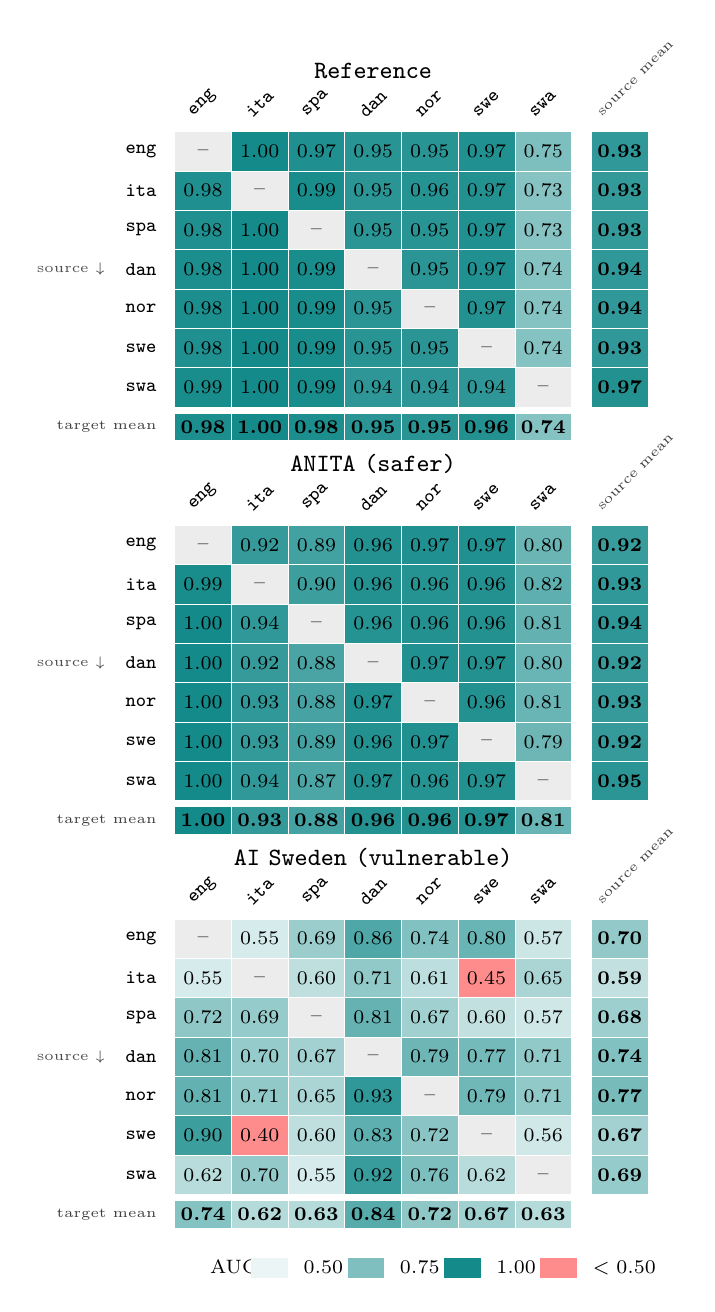
\begin{tikzpicture}[x=0.72cm,y=0.50cm]
\node[font=\small,align=center,text width=7.0cm] at (3.5,1.55) {\texttt{Reference}};
\node[font=\tiny,text=black!70,anchor=east] at (-1.05,-3.5) {source $\downarrow$};
\node[rotate=45,anchor=west,font=\scriptsize] at (0.18,0.25) {\texttt{eng}};
\node[rotate=45,anchor=west,font=\scriptsize] at (1.18,0.25) {\texttt{ita}};
\node[rotate=45,anchor=west,font=\scriptsize] at (2.18,0.25) {\texttt{spa}};
\node[rotate=45,anchor=west,font=\scriptsize] at (3.18,0.25) {\texttt{dan}};
\node[rotate=45,anchor=west,font=\scriptsize] at (4.18,0.25) {\texttt{nor}};
\node[rotate=45,anchor=west,font=\scriptsize] at (5.18,0.25) {\texttt{swe}};
\node[rotate=45,anchor=west,font=\scriptsize] at (6.18,0.25) {\texttt{swa}};
\node[rotate=45,anchor=west,font=\tiny,text=black!75] at (7.38,0.25) {source mean};
\node[anchor=east,font=\scriptsize] at (-0.15,-0.5) {\texttt{eng}};
\fill[gray!15] (0,0) rectangle ++(1,-1);
\draw[white,line width=0.25pt] (0,0) rectangle ++(1,-1);
\node[font=\scriptsize] at (0.5,-0.5) {--};
\fill[teal!92!white] (1,0) rectangle ++(1,-1);
\draw[white,line width=0.25pt] (1,0) rectangle ++(1,-1);
\node[font=\scriptsize] at (1.5,-0.5) {1.00};
\fill[teal!88!white] (2,0) rectangle ++(1,-1);
\draw[white,line width=0.25pt] (2,0) rectangle ++(1,-1);
\node[font=\scriptsize] at (2.5,-0.5) {0.97};
\fill[teal!84!white] (3,0) rectangle ++(1,-1);
\draw[white,line width=0.25pt] (3,0) rectangle ++(1,-1);
\node[font=\scriptsize] at (3.5,-0.5) {0.95};
\fill[teal!84!white] (4,0) rectangle ++(1,-1);
\draw[white,line width=0.25pt] (4,0) rectangle ++(1,-1);
\node[font=\scriptsize] at (4.5,-0.5) {0.95};
\fill[teal!87!white] (5,0) rectangle ++(1,-1);
\draw[white,line width=0.25pt] (5,0) rectangle ++(1,-1);
\node[font=\scriptsize] at (5.5,-0.5) {0.97};
\fill[teal!51!white] (6,0) rectangle ++(1,-1);
\draw[white,line width=0.25pt] (6,0) rectangle ++(1,-1);
\node[font=\scriptsize] at (6.5,-0.5) {0.75};
\fill[teal!81!white] (7.35,0) rectangle ++(1,-1);
\draw[white,line width=0.25pt] (7.35,0) rectangle ++(1,-1);
\node[font=\scriptsize\bfseries] at (7.85,-0.5) {0.93};
\node[anchor=east,font=\scriptsize] at (-0.15,-1.5) {\texttt{ita}};
\fill[teal!88!white] (0,-1) rectangle ++(1,-1);
\draw[white,line width=0.25pt] (0,-1) rectangle ++(1,-1);
\node[font=\scriptsize] at (0.5,-1.5) {0.98};
\fill[gray!15] (1,-1) rectangle ++(1,-1);
\draw[white,line width=0.25pt] (1,-1) rectangle ++(1,-1);
\node[font=\scriptsize] at (1.5,-1.5) {--};
\fill[teal!90!white] (2,-1) rectangle ++(1,-1);
\draw[white,line width=0.25pt] (2,-1) rectangle ++(1,-1);
\node[font=\scriptsize] at (2.5,-1.5) {0.99};
\fill[teal!83!white] (3,-1) rectangle ++(1,-1);
\draw[white,line width=0.25pt] (3,-1) rectangle ++(1,-1);
\node[font=\scriptsize] at (3.5,-1.5) {0.95};
\fill[teal!85!white] (4,-1) rectangle ++(1,-1);
\draw[white,line width=0.25pt] (4,-1) rectangle ++(1,-1);
\node[font=\scriptsize] at (4.5,-1.5) {0.96};
\fill[teal!86!white] (5,-1) rectangle ++(1,-1);
\draw[white,line width=0.25pt] (5,-1) rectangle ++(1,-1);
\node[font=\scriptsize] at (5.5,-1.5) {0.97};
\fill[teal!47!white] (6,-1) rectangle ++(1,-1);
\draw[white,line width=0.25pt] (6,-1) rectangle ++(1,-1);
\node[font=\scriptsize] at (6.5,-1.5) {0.73};
\fill[teal!80!white] (7.35,-1) rectangle ++(1,-1);
\draw[white,line width=0.25pt] (7.35,-1) rectangle ++(1,-1);
\node[font=\scriptsize\bfseries] at (7.85,-1.5) {0.93};
\node[anchor=east,font=\scriptsize] at (-0.15,-2.5) {\texttt{spa}};
\fill[teal!88!white] (0,-2) rectangle ++(1,-1);
\draw[white,line width=0.25pt] (0,-2) rectangle ++(1,-1);
\node[font=\scriptsize] at (0.5,-2.5) {0.98};
\fill[teal!92!white] (1,-2) rectangle ++(1,-1);
\draw[white,line width=0.25pt] (1,-2) rectangle ++(1,-1);
\node[font=\scriptsize] at (1.5,-2.5) {1.00};
\fill[gray!15] (2,-2) rectangle ++(1,-1);
\draw[white,line width=0.25pt] (2,-2) rectangle ++(1,-1);
\node[font=\scriptsize] at (2.5,-2.5) {--};
\fill[teal!83!white] (3,-2) rectangle ++(1,-1);
\draw[white,line width=0.25pt] (3,-2) rectangle ++(1,-1);
\node[font=\scriptsize] at (3.5,-2.5) {0.95};
\fill[teal!84!white] (4,-2) rectangle ++(1,-1);
\draw[white,line width=0.25pt] (4,-2) rectangle ++(1,-1);
\node[font=\scriptsize] at (4.5,-2.5) {0.95};
\fill[teal!87!white] (5,-2) rectangle ++(1,-1);
\draw[white,line width=0.25pt] (5,-2) rectangle ++(1,-1);
\node[font=\scriptsize] at (5.5,-2.5) {0.97};
\fill[teal!47!white] (6,-2) rectangle ++(1,-1);
\draw[white,line width=0.25pt] (6,-2) rectangle ++(1,-1);
\node[font=\scriptsize] at (6.5,-2.5) {0.73};
\fill[teal!80!white] (7.35,-2) rectangle ++(1,-1);
\draw[white,line width=0.25pt] (7.35,-2) rectangle ++(1,-1);
\node[font=\scriptsize\bfseries] at (7.85,-2.5) {0.93};
\node[anchor=east,font=\scriptsize] at (-0.15,-3.5) {\texttt{dan}};
\fill[teal!89!white] (0,-3) rectangle ++(1,-1);
\draw[white,line width=0.25pt] (0,-3) rectangle ++(1,-1);
\node[font=\scriptsize] at (0.5,-3.5) {0.98};
\fill[teal!92!white] (1,-3) rectangle ++(1,-1);
\draw[white,line width=0.25pt] (1,-3) rectangle ++(1,-1);
\node[font=\scriptsize] at (1.5,-3.5) {1.00};
\fill[teal!90!white] (2,-3) rectangle ++(1,-1);
\draw[white,line width=0.25pt] (2,-3) rectangle ++(1,-1);
\node[font=\scriptsize] at (2.5,-3.5) {0.99};
\fill[gray!15] (3,-3) rectangle ++(1,-1);
\draw[white,line width=0.25pt] (3,-3) rectangle ++(1,-1);
\node[font=\scriptsize] at (3.5,-3.5) {--};
\fill[teal!83!white] (4,-3) rectangle ++(1,-1);
\draw[white,line width=0.25pt] (4,-3) rectangle ++(1,-1);
\node[font=\scriptsize] at (4.5,-3.5) {0.95};
\fill[teal!87!white] (5,-3) rectangle ++(1,-1);
\draw[white,line width=0.25pt] (5,-3) rectangle ++(1,-1);
\node[font=\scriptsize] at (5.5,-3.5) {0.97};
\fill[teal!48!white] (6,-3) rectangle ++(1,-1);
\draw[white,line width=0.25pt] (6,-3) rectangle ++(1,-1);
\node[font=\scriptsize] at (6.5,-3.5) {0.74};
\fill[teal!81!white] (7.35,-3) rectangle ++(1,-1);
\draw[white,line width=0.25pt] (7.35,-3) rectangle ++(1,-1);
\node[font=\scriptsize\bfseries] at (7.85,-3.5) {0.94};
\node[anchor=east,font=\scriptsize] at (-0.15,-4.5) {\texttt{nor}};
\fill[teal!89!white] (0,-4) rectangle ++(1,-1);
\draw[white,line width=0.25pt] (0,-4) rectangle ++(1,-1);
\node[font=\scriptsize] at (0.5,-4.5) {0.98};
\fill[teal!92!white] (1,-4) rectangle ++(1,-1);
\draw[white,line width=0.25pt] (1,-4) rectangle ++(1,-1);
\node[font=\scriptsize] at (1.5,-4.5) {1.00};
\fill[teal!90!white] (2,-4) rectangle ++(1,-1);
\draw[white,line width=0.25pt] (2,-4) rectangle ++(1,-1);
\node[font=\scriptsize] at (2.5,-4.5) {0.99};
\fill[teal!83!white] (3,-4) rectangle ++(1,-1);
\draw[white,line width=0.25pt] (3,-4) rectangle ++(1,-1);
\node[font=\scriptsize] at (3.5,-4.5) {0.95};
\fill[gray!15] (4,-4) rectangle ++(1,-1);
\draw[white,line width=0.25pt] (4,-4) rectangle ++(1,-1);
\node[font=\scriptsize] at (4.5,-4.5) {--};
\fill[teal!86!white] (5,-4) rectangle ++(1,-1);
\draw[white,line width=0.25pt] (5,-4) rectangle ++(1,-1);
\node[font=\scriptsize] at (5.5,-4.5) {0.97};
\fill[teal!48!white] (6,-4) rectangle ++(1,-1);
\draw[white,line width=0.25pt] (6,-4) rectangle ++(1,-1);
\node[font=\scriptsize] at (6.5,-4.5) {0.74};
\fill[teal!81!white] (7.35,-4) rectangle ++(1,-1);
\draw[white,line width=0.25pt] (7.35,-4) rectangle ++(1,-1);
\node[font=\scriptsize\bfseries] at (7.85,-4.5) {0.94};
\node[anchor=east,font=\scriptsize] at (-0.15,-5.5) {\texttt{swe}};
\fill[teal!88!white] (0,-5) rectangle ++(1,-1);
\draw[white,line width=0.25pt] (0,-5) rectangle ++(1,-1);
\node[font=\scriptsize] at (0.5,-5.5) {0.98};
\fill[teal!92!white] (1,-5) rectangle ++(1,-1);
\draw[white,line width=0.25pt] (1,-5) rectangle ++(1,-1);
\node[font=\scriptsize] at (1.5,-5.5) {1.00};
\fill[teal!90!white] (2,-5) rectangle ++(1,-1);
\draw[white,line width=0.25pt] (2,-5) rectangle ++(1,-1);
\node[font=\scriptsize] at (2.5,-5.5) {0.99};
\fill[teal!84!white] (3,-5) rectangle ++(1,-1);
\draw[white,line width=0.25pt] (3,-5) rectangle ++(1,-1);
\node[font=\scriptsize] at (3.5,-5.5) {0.95};
\fill[teal!83!white] (4,-5) rectangle ++(1,-1);
\draw[white,line width=0.25pt] (4,-5) rectangle ++(1,-1);
\node[font=\scriptsize] at (4.5,-5.5) {0.95};
\fill[gray!15] (5,-5) rectangle ++(1,-1);
\draw[white,line width=0.25pt] (5,-5) rectangle ++(1,-1);
\node[font=\scriptsize] at (5.5,-5.5) {--};
\fill[teal!48!white] (6,-5) rectangle ++(1,-1);
\draw[white,line width=0.25pt] (6,-5) rectangle ++(1,-1);
\node[font=\scriptsize] at (6.5,-5.5) {0.74};
\fill[teal!81!white] (7.35,-5) rectangle ++(1,-1);
\draw[white,line width=0.25pt] (7.35,-5) rectangle ++(1,-1);
\node[font=\scriptsize\bfseries] at (7.85,-5.5) {0.93};
\node[anchor=east,font=\scriptsize] at (-0.15,-6.5) {\texttt{swa}};
\fill[teal!90!white] (0,-6) rectangle ++(1,-1);
\draw[white,line width=0.25pt] (0,-6) rectangle ++(1,-1);
\node[font=\scriptsize] at (0.5,-6.5) {0.99};
\fill[teal!92!white] (1,-6) rectangle ++(1,-1);
\draw[white,line width=0.25pt] (1,-6) rectangle ++(1,-1);
\node[font=\scriptsize] at (1.5,-6.5) {1.00};
\fill[teal!90!white] (2,-6) rectangle ++(1,-1);
\draw[white,line width=0.25pt] (2,-6) rectangle ++(1,-1);
\node[font=\scriptsize] at (2.5,-6.5) {0.99};
\fill[teal!82!white] (3,-6) rectangle ++(1,-1);
\draw[white,line width=0.25pt] (3,-6) rectangle ++(1,-1);
\node[font=\scriptsize] at (3.5,-6.5) {0.94};
\fill[teal!82!white] (4,-6) rectangle ++(1,-1);
\draw[white,line width=0.25pt] (4,-6) rectangle ++(1,-1);
\node[font=\scriptsize] at (4.5,-6.5) {0.94};
\fill[teal!82!white] (5,-6) rectangle ++(1,-1);
\draw[white,line width=0.25pt] (5,-6) rectangle ++(1,-1);
\node[font=\scriptsize] at (5.5,-6.5) {0.94};
\fill[gray!15] (6,-6) rectangle ++(1,-1);
\draw[white,line width=0.25pt] (6,-6) rectangle ++(1,-1);
\node[font=\scriptsize] at (6.5,-6.5) {--};
\fill[teal!86!white] (7.35,-6) rectangle ++(1,-1);
\draw[white,line width=0.25pt] (7.35,-6) rectangle ++(1,-1);
\node[font=\scriptsize\bfseries] at (7.85,-6.5) {0.97};
\node[anchor=east,font=\tiny,text=black!75] at (-0.15,-7.5) {target mean};
\fill[teal!89!white] (0,-7.15) rectangle ++(1,-0.70);
\draw[white,line width=0.25pt] (0,-7.15) rectangle ++(1,-0.70);
\node[font=\scriptsize\bfseries] at (0.5,-7.5) {0.98};
\fill[teal!92!white] (1,-7.15) rectangle ++(1,-0.70);
\draw[white,line width=0.25pt] (1,-7.15) rectangle ++(1,-0.70);
\node[font=\scriptsize\bfseries] at (1.5,-7.5) {1.00};
\fill[teal!89!white] (2,-7.15) rectangle ++(1,-0.70);
\draw[white,line width=0.25pt] (2,-7.15) rectangle ++(1,-0.70);
\node[font=\scriptsize\bfseries] at (2.5,-7.5) {0.98};
\fill[teal!83!white] (3,-7.15) rectangle ++(1,-0.70);
\draw[white,line width=0.25pt] (3,-7.15) rectangle ++(1,-0.70);
\node[font=\scriptsize\bfseries] at (3.5,-7.5) {0.95};
\fill[teal!84!white] (4,-7.15) rectangle ++(1,-0.70);
\draw[white,line width=0.25pt] (4,-7.15) rectangle ++(1,-0.70);
\node[font=\scriptsize\bfseries] at (4.5,-7.5) {0.95};
\fill[teal!86!white] (5,-7.15) rectangle ++(1,-0.70);
\draw[white,line width=0.25pt] (5,-7.15) rectangle ++(1,-0.70);
\node[font=\scriptsize\bfseries] at (5.5,-7.5) {0.96};
\fill[teal!48!white] (6,-7.15) rectangle ++(1,-0.70);
\draw[white,line width=0.25pt] (6,-7.15) rectangle ++(1,-0.70);
\node[font=\scriptsize\bfseries] at (6.5,-7.5) {0.74};
\node[font=\small,align=center,text width=7.0cm] at (3.5,-8.45) {\texttt{ANITA (safer)}};
\node[font=\tiny,text=black!70,anchor=east] at (-1.05,-13.5) {source $\downarrow$};
\node[rotate=45,anchor=west,font=\scriptsize] at (0.18,-9.75) {\texttt{eng}};
\node[rotate=45,anchor=west,font=\scriptsize] at (1.18,-9.75) {\texttt{ita}};
\node[rotate=45,anchor=west,font=\scriptsize] at (2.18,-9.75) {\texttt{spa}};
\node[rotate=45,anchor=west,font=\scriptsize] at (3.18,-9.75) {\texttt{dan}};
\node[rotate=45,anchor=west,font=\scriptsize] at (4.18,-9.75) {\texttt{nor}};
\node[rotate=45,anchor=west,font=\scriptsize] at (5.18,-9.75) {\texttt{swe}};
\node[rotate=45,anchor=west,font=\scriptsize] at (6.18,-9.75) {\texttt{swa}};
\node[rotate=45,anchor=west,font=\tiny,text=black!75] at (7.38,-9.75) {source mean};
\node[anchor=east,font=\scriptsize] at (-0.15,-10.5) {\texttt{eng}};
\fill[gray!15] (0,-10) rectangle ++(1,-1);
\draw[white,line width=0.25pt] (0,-10) rectangle ++(1,-1);
\node[font=\scriptsize] at (0.5,-10.5) {--};
\fill[teal!79!white] (1,-10) rectangle ++(1,-1);
\draw[white,line width=0.25pt] (1,-10) rectangle ++(1,-1);
\node[font=\scriptsize] at (1.5,-10.5) {0.92};
\fill[teal!74!white] (2,-10) rectangle ++(1,-1);
\draw[white,line width=0.25pt] (2,-10) rectangle ++(1,-1);
\node[font=\scriptsize] at (2.5,-10.5) {0.89};
\fill[teal!86!white] (3,-10) rectangle ++(1,-1);
\draw[white,line width=0.25pt] (3,-10) rectangle ++(1,-1);
\node[font=\scriptsize] at (3.5,-10.5) {0.96};
\fill[teal!87!white] (4,-10) rectangle ++(1,-1);
\draw[white,line width=0.25pt] (4,-10) rectangle ++(1,-1);
\node[font=\scriptsize] at (4.5,-10.5) {0.97};
\fill[teal!87!white] (5,-10) rectangle ++(1,-1);
\draw[white,line width=0.25pt] (5,-10) rectangle ++(1,-1);
\node[font=\scriptsize] at (5.5,-10.5) {0.97};
\fill[teal!58!white] (6,-10) rectangle ++(1,-1);
\draw[white,line width=0.25pt] (6,-10) rectangle ++(1,-1);
\node[font=\scriptsize] at (6.5,-10.5) {0.80};
\fill[teal!78!white] (7.35,-10) rectangle ++(1,-1);
\draw[white,line width=0.25pt] (7.35,-10) rectangle ++(1,-1);
\node[font=\scriptsize\bfseries] at (7.85,-10.5) {0.92};
\node[anchor=east,font=\scriptsize] at (-0.15,-11.5) {\texttt{ita}};
\fill[teal!90!white] (0,-11) rectangle ++(1,-1);
\draw[white,line width=0.25pt] (0,-11) rectangle ++(1,-1);
\node[font=\scriptsize] at (0.5,-11.5) {0.99};
\fill[gray!15] (1,-11) rectangle ++(1,-1);
\draw[white,line width=0.25pt] (1,-11) rectangle ++(1,-1);
\node[font=\scriptsize] at (1.5,-11.5) {--};
\fill[teal!76!white] (2,-11) rectangle ++(1,-1);
\draw[white,line width=0.25pt] (2,-11) rectangle ++(1,-1);
\node[font=\scriptsize] at (2.5,-11.5) {0.90};
\fill[teal!86!white] (3,-11) rectangle ++(1,-1);
\draw[white,line width=0.25pt] (3,-11) rectangle ++(1,-1);
\node[font=\scriptsize] at (3.5,-11.5) {0.96};
\fill[teal!85!white] (4,-11) rectangle ++(1,-1);
\draw[white,line width=0.25pt] (4,-11) rectangle ++(1,-1);
\node[font=\scriptsize] at (4.5,-11.5) {0.96};
\fill[teal!86!white] (5,-11) rectangle ++(1,-1);
\draw[white,line width=0.25pt] (5,-11) rectangle ++(1,-1);
\node[font=\scriptsize] at (5.5,-11.5) {0.96};
\fill[teal!63!white] (6,-11) rectangle ++(1,-1);
\draw[white,line width=0.25pt] (6,-11) rectangle ++(1,-1);
\node[font=\scriptsize] at (6.5,-11.5) {0.82};
\fill[teal!81!white] (7.35,-11) rectangle ++(1,-1);
\draw[white,line width=0.25pt] (7.35,-11) rectangle ++(1,-1);
\node[font=\scriptsize\bfseries] at (7.85,-11.5) {0.93};
\node[anchor=east,font=\scriptsize] at (-0.15,-12.5) {\texttt{spa}};
\fill[teal!92!white] (0,-12) rectangle ++(1,-1);
\draw[white,line width=0.25pt] (0,-12) rectangle ++(1,-1);
\node[font=\scriptsize] at (0.5,-12.5) {1.00};
\fill[teal!81!white] (1,-12) rectangle ++(1,-1);
\draw[white,line width=0.25pt] (1,-12) rectangle ++(1,-1);
\node[font=\scriptsize] at (1.5,-12.5) {0.94};
\fill[gray!15] (2,-12) rectangle ++(1,-1);
\draw[white,line width=0.25pt] (2,-12) rectangle ++(1,-1);
\node[font=\scriptsize] at (2.5,-12.5) {--};
\fill[teal!85!white] (3,-12) rectangle ++(1,-1);
\draw[white,line width=0.25pt] (3,-12) rectangle ++(1,-1);
\node[font=\scriptsize] at (3.5,-12.5) {0.96};
\fill[teal!86!white] (4,-12) rectangle ++(1,-1);
\draw[white,line width=0.25pt] (4,-12) rectangle ++(1,-1);
\node[font=\scriptsize] at (4.5,-12.5) {0.96};
\fill[teal!86!white] (5,-12) rectangle ++(1,-1);
\draw[white,line width=0.25pt] (5,-12) rectangle ++(1,-1);
\node[font=\scriptsize] at (5.5,-12.5) {0.96};
\fill[teal!61!white] (6,-12) rectangle ++(1,-1);
\draw[white,line width=0.25pt] (6,-12) rectangle ++(1,-1);
\node[font=\scriptsize] at (6.5,-12.5) {0.81};
\fill[teal!82!white] (7.35,-12) rectangle ++(1,-1);
\draw[white,line width=0.25pt] (7.35,-12) rectangle ++(1,-1);
\node[font=\scriptsize\bfseries] at (7.85,-12.5) {0.94};
\node[anchor=east,font=\scriptsize] at (-0.15,-13.5) {\texttt{dan}};
\fill[teal!92!white] (0,-13) rectangle ++(1,-1);
\draw[white,line width=0.25pt] (0,-13) rectangle ++(1,-1);
\node[font=\scriptsize] at (0.5,-13.5) {1.00};
\fill[teal!79!white] (1,-13) rectangle ++(1,-1);
\draw[white,line width=0.25pt] (1,-13) rectangle ++(1,-1);
\node[font=\scriptsize] at (1.5,-13.5) {0.92};
\fill[teal!71!white] (2,-13) rectangle ++(1,-1);
\draw[white,line width=0.25pt] (2,-13) rectangle ++(1,-1);
\node[font=\scriptsize] at (2.5,-13.5) {0.88};
\fill[gray!15] (3,-13) rectangle ++(1,-1);
\draw[white,line width=0.25pt] (3,-13) rectangle ++(1,-1);
\node[font=\scriptsize] at (3.5,-13.5) {--};
\fill[teal!87!white] (4,-13) rectangle ++(1,-1);
\draw[white,line width=0.25pt] (4,-13) rectangle ++(1,-1);
\node[font=\scriptsize] at (4.5,-13.5) {0.97};
\fill[teal!86!white] (5,-13) rectangle ++(1,-1);
\draw[white,line width=0.25pt] (5,-13) rectangle ++(1,-1);
\node[font=\scriptsize] at (5.5,-13.5) {0.97};
\fill[teal!59!white] (6,-13) rectangle ++(1,-1);
\draw[white,line width=0.25pt] (6,-13) rectangle ++(1,-1);
\node[font=\scriptsize] at (6.5,-13.5) {0.80};
\fill[teal!79!white] (7.35,-13) rectangle ++(1,-1);
\draw[white,line width=0.25pt] (7.35,-13) rectangle ++(1,-1);
\node[font=\scriptsize\bfseries] at (7.85,-13.5) {0.92};
\node[anchor=east,font=\scriptsize] at (-0.15,-14.5) {\texttt{nor}};
\fill[teal!92!white] (0,-14) rectangle ++(1,-1);
\draw[white,line width=0.25pt] (0,-14) rectangle ++(1,-1);
\node[font=\scriptsize] at (0.5,-14.5) {1.00};
\fill[teal!81!white] (1,-14) rectangle ++(1,-1);
\draw[white,line width=0.25pt] (1,-14) rectangle ++(1,-1);
\node[font=\scriptsize] at (1.5,-14.5) {0.93};
\fill[teal!72!white] (2,-14) rectangle ++(1,-1);
\draw[white,line width=0.25pt] (2,-14) rectangle ++(1,-1);
\node[font=\scriptsize] at (2.5,-14.5) {0.88};
\fill[teal!87!white] (3,-14) rectangle ++(1,-1);
\draw[white,line width=0.25pt] (3,-14) rectangle ++(1,-1);
\node[font=\scriptsize] at (3.5,-14.5) {0.97};
\fill[gray!15] (4,-14) rectangle ++(1,-1);
\draw[white,line width=0.25pt] (4,-14) rectangle ++(1,-1);
\node[font=\scriptsize] at (4.5,-14.5) {--};
\fill[teal!86!white] (5,-14) rectangle ++(1,-1);
\draw[white,line width=0.25pt] (5,-14) rectangle ++(1,-1);
\node[font=\scriptsize] at (5.5,-14.5) {0.96};
\fill[teal!59!white] (6,-14) rectangle ++(1,-1);
\draw[white,line width=0.25pt] (6,-14) rectangle ++(1,-1);
\node[font=\scriptsize] at (6.5,-14.5) {0.81};
\fill[teal!79!white] (7.35,-14) rectangle ++(1,-1);
\draw[white,line width=0.25pt] (7.35,-14) rectangle ++(1,-1);
\node[font=\scriptsize\bfseries] at (7.85,-14.5) {0.93};
\node[anchor=east,font=\scriptsize] at (-0.15,-15.5) {\texttt{swe}};
\fill[teal!92!white] (0,-15) rectangle ++(1,-1);
\draw[white,line width=0.25pt] (0,-15) rectangle ++(1,-1);
\node[font=\scriptsize] at (0.5,-15.5) {1.00};
\fill[teal!80!white] (1,-15) rectangle ++(1,-1);
\draw[white,line width=0.25pt] (1,-15) rectangle ++(1,-1);
\node[font=\scriptsize] at (1.5,-15.5) {0.93};
\fill[teal!73!white] (2,-15) rectangle ++(1,-1);
\draw[white,line width=0.25pt] (2,-15) rectangle ++(1,-1);
\node[font=\scriptsize] at (2.5,-15.5) {0.89};
\fill[teal!86!white] (3,-15) rectangle ++(1,-1);
\draw[white,line width=0.25pt] (3,-15) rectangle ++(1,-1);
\node[font=\scriptsize] at (3.5,-15.5) {0.96};
\fill[teal!87!white] (4,-15) rectangle ++(1,-1);
\draw[white,line width=0.25pt] (4,-15) rectangle ++(1,-1);
\node[font=\scriptsize] at (4.5,-15.5) {0.97};
\fill[gray!15] (5,-15) rectangle ++(1,-1);
\draw[white,line width=0.25pt] (5,-15) rectangle ++(1,-1);
\node[font=\scriptsize] at (5.5,-15.5) {--};
\fill[teal!57!white] (6,-15) rectangle ++(1,-1);
\draw[white,line width=0.25pt] (6,-15) rectangle ++(1,-1);
\node[font=\scriptsize] at (6.5,-15.5) {0.79};
\fill[teal!79!white] (7.35,-15) rectangle ++(1,-1);
\draw[white,line width=0.25pt] (7.35,-15) rectangle ++(1,-1);
\node[font=\scriptsize\bfseries] at (7.85,-15.5) {0.92};
\node[anchor=east,font=\scriptsize] at (-0.15,-16.5) {\texttt{swa}};
\fill[teal!92!white] (0,-16) rectangle ++(1,-1);
\draw[white,line width=0.25pt] (0,-16) rectangle ++(1,-1);
\node[font=\scriptsize] at (0.5,-16.5) {1.00};
\fill[teal!81!white] (1,-16) rectangle ++(1,-1);
\draw[white,line width=0.25pt] (1,-16) rectangle ++(1,-1);
\node[font=\scriptsize] at (1.5,-16.5) {0.94};
\fill[teal!70!white] (2,-16) rectangle ++(1,-1);
\draw[white,line width=0.25pt] (2,-16) rectangle ++(1,-1);
\node[font=\scriptsize] at (2.5,-16.5) {0.87};
\fill[teal!86!white] (3,-16) rectangle ++(1,-1);
\draw[white,line width=0.25pt] (3,-16) rectangle ++(1,-1);
\node[font=\scriptsize] at (3.5,-16.5) {0.97};
\fill[teal!85!white] (4,-16) rectangle ++(1,-1);
\draw[white,line width=0.25pt] (4,-16) rectangle ++(1,-1);
\node[font=\scriptsize] at (4.5,-16.5) {0.96};
\fill[teal!86!white] (5,-16) rectangle ++(1,-1);
\draw[white,line width=0.25pt] (5,-16) rectangle ++(1,-1);
\node[font=\scriptsize] at (5.5,-16.5) {0.97};
\fill[gray!15] (6,-16) rectangle ++(1,-1);
\draw[white,line width=0.25pt] (6,-16) rectangle ++(1,-1);
\node[font=\scriptsize] at (6.5,-16.5) {--};
\fill[teal!83!white] (7.35,-16) rectangle ++(1,-1);
\draw[white,line width=0.25pt] (7.35,-16) rectangle ++(1,-1);
\node[font=\scriptsize\bfseries] at (7.85,-16.5) {0.95};
\node[anchor=east,font=\tiny,text=black!75] at (-0.15,-17.5) {target mean};
\fill[teal!92!white] (0,-17.15) rectangle ++(1,-0.70);
\draw[white,line width=0.25pt] (0,-17.15) rectangle ++(1,-0.70);
\node[font=\scriptsize\bfseries] at (0.5,-17.5) {1.00};
\fill[teal!80!white] (1,-17.15) rectangle ++(1,-0.70);
\draw[white,line width=0.25pt] (1,-17.15) rectangle ++(1,-0.70);
\node[font=\scriptsize\bfseries] at (1.5,-17.5) {0.93};
\fill[teal!73!white] (2,-17.15) rectangle ++(1,-0.70);
\draw[white,line width=0.25pt] (2,-17.15) rectangle ++(1,-0.70);
\node[font=\scriptsize\bfseries] at (2.5,-17.5) {0.88};
\fill[teal!86!white] (3,-17.15) rectangle ++(1,-0.70);
\draw[white,line width=0.25pt] (3,-17.15) rectangle ++(1,-0.70);
\node[font=\scriptsize\bfseries] at (3.5,-17.5) {0.96};
\fill[teal!86!white] (4,-17.15) rectangle ++(1,-0.70);
\draw[white,line width=0.25pt] (4,-17.15) rectangle ++(1,-0.70);
\node[font=\scriptsize\bfseries] at (4.5,-17.5) {0.96};
\fill[teal!86!white] (5,-17.15) rectangle ++(1,-0.70);
\draw[white,line width=0.25pt] (5,-17.15) rectangle ++(1,-0.70);
\node[font=\scriptsize\bfseries] at (5.5,-17.5) {0.97};
\fill[teal!59!white] (6,-17.15) rectangle ++(1,-0.70);
\draw[white,line width=0.25pt] (6,-17.15) rectangle ++(1,-0.70);
\node[font=\scriptsize\bfseries] at (6.5,-17.5) {0.81};
\node[font=\small,align=center,text width=7.0cm] at (3.5,-18.45) {\texttt{AI Sweden (vulnerable)}};
\node[font=\tiny,text=black!70,anchor=east] at (-1.05,-23.5) {source $\downarrow$};
\node[rotate=45,anchor=west,font=\scriptsize] at (0.18,-19.75) {\texttt{eng}};
\node[rotate=45,anchor=west,font=\scriptsize] at (1.18,-19.75) {\texttt{ita}};
\node[rotate=45,anchor=west,font=\scriptsize] at (2.18,-19.75) {\texttt{spa}};
\node[rotate=45,anchor=west,font=\scriptsize] at (3.18,-19.75) {\texttt{dan}};
\node[rotate=45,anchor=west,font=\scriptsize] at (4.18,-19.75) {\texttt{nor}};
\node[rotate=45,anchor=west,font=\scriptsize] at (5.18,-19.75) {\texttt{swe}};
\node[rotate=45,anchor=west,font=\scriptsize] at (6.18,-19.75) {\texttt{swa}};
\node[rotate=45,anchor=west,font=\tiny,text=black!75] at (7.38,-19.75) {source mean};
\node[anchor=east,font=\scriptsize] at (-0.15,-20.5) {\texttt{eng}};
\fill[gray!15] (0,-20) rectangle ++(1,-1);
\draw[white,line width=0.25pt] (0,-20) rectangle ++(1,-1);
\node[font=\scriptsize] at (0.5,-20.5) {--};
\fill[teal!16!white] (1,-20) rectangle ++(1,-1);
\draw[white,line width=0.25pt] (1,-20) rectangle ++(1,-1);
\node[font=\scriptsize] at (1.5,-20.5) {0.55};
\fill[teal!39!white] (2,-20) rectangle ++(1,-1);
\draw[white,line width=0.25pt] (2,-20) rectangle ++(1,-1);
\node[font=\scriptsize] at (2.5,-20.5) {0.69};
\fill[teal!69!white] (3,-20) rectangle ++(1,-1);
\draw[white,line width=0.25pt] (3,-20) rectangle ++(1,-1);
\node[font=\scriptsize] at (3.5,-20.5) {0.86};
\fill[teal!49!white] (4,-20) rectangle ++(1,-1);
\draw[white,line width=0.25pt] (4,-20) rectangle ++(1,-1);
\node[font=\scriptsize] at (4.5,-20.5) {0.74};
\fill[teal!59!white] (5,-20) rectangle ++(1,-1);
\draw[white,line width=0.25pt] (5,-20) rectangle ++(1,-1);
\node[font=\scriptsize] at (5.5,-20.5) {0.80};
\fill[teal!20!white] (6,-20) rectangle ++(1,-1);
\draw[white,line width=0.25pt] (6,-20) rectangle ++(1,-1);
\node[font=\scriptsize] at (6.5,-20.5) {0.57};
\fill[teal!42!white] (7.35,-20) rectangle ++(1,-1);
\draw[white,line width=0.25pt] (7.35,-20) rectangle ++(1,-1);
\node[font=\scriptsize\bfseries] at (7.85,-20.5) {0.70};
\node[anchor=east,font=\scriptsize] at (-0.15,-21.5) {\texttt{ita}};
\fill[teal!16!white] (0,-21) rectangle ++(1,-1);
\draw[white,line width=0.25pt] (0,-21) rectangle ++(1,-1);
\node[font=\scriptsize] at (0.5,-21.5) {0.55};
\fill[gray!15] (1,-21) rectangle ++(1,-1);
\draw[white,line width=0.25pt] (1,-21) rectangle ++(1,-1);
\node[font=\scriptsize] at (1.5,-21.5) {--};
\fill[teal!25!white] (2,-21) rectangle ++(1,-1);
\draw[white,line width=0.25pt] (2,-21) rectangle ++(1,-1);
\node[font=\scriptsize] at (2.5,-21.5) {0.60};
\fill[teal!43!white] (3,-21) rectangle ++(1,-1);
\draw[white,line width=0.25pt] (3,-21) rectangle ++(1,-1);
\node[font=\scriptsize] at (3.5,-21.5) {0.71};
\fill[teal!26!white] (4,-21) rectangle ++(1,-1);
\draw[white,line width=0.25pt] (4,-21) rectangle ++(1,-1);
\node[font=\scriptsize] at (4.5,-21.5) {0.61};
\fill[red!45!white] (5,-21) rectangle ++(1,-1);
\draw[white,line width=0.25pt] (5,-21) rectangle ++(1,-1);
\node[font=\scriptsize] at (5.5,-21.5) {0.45};
\fill[teal!33!white] (6,-21) rectangle ++(1,-1);
\draw[white,line width=0.25pt] (6,-21) rectangle ++(1,-1);
\node[font=\scriptsize] at (6.5,-21.5) {0.65};
\fill[teal!24!white] (7.35,-21) rectangle ++(1,-1);
\draw[white,line width=0.25pt] (7.35,-21) rectangle ++(1,-1);
\node[font=\scriptsize\bfseries] at (7.85,-21.5) {0.59};
\node[anchor=east,font=\scriptsize] at (-0.15,-22.5) {\texttt{spa}};
\fill[teal!44!white] (0,-22) rectangle ++(1,-1);
\draw[white,line width=0.25pt] (0,-22) rectangle ++(1,-1);
\node[font=\scriptsize] at (0.5,-22.5) {0.72};
\fill[teal!41!white] (1,-22) rectangle ++(1,-1);
\draw[white,line width=0.25pt] (1,-22) rectangle ++(1,-1);
\node[font=\scriptsize] at (1.5,-22.5) {0.69};
\fill[gray!15] (2,-22) rectangle ++(1,-1);
\draw[white,line width=0.25pt] (2,-22) rectangle ++(1,-1);
\node[font=\scriptsize] at (2.5,-22.5) {--};
\fill[teal!60!white] (3,-22) rectangle ++(1,-1);
\draw[white,line width=0.25pt] (3,-22) rectangle ++(1,-1);
\node[font=\scriptsize] at (3.5,-22.5) {0.81};
\fill[teal!37!white] (4,-22) rectangle ++(1,-1);
\draw[white,line width=0.25pt] (4,-22) rectangle ++(1,-1);
\node[font=\scriptsize] at (4.5,-22.5) {0.67};
\fill[teal!24!white] (5,-22) rectangle ++(1,-1);
\draw[white,line width=0.25pt] (5,-22) rectangle ++(1,-1);
\node[font=\scriptsize] at (5.5,-22.5) {0.60};
\fill[teal!19!white] (6,-22) rectangle ++(1,-1);
\draw[white,line width=0.25pt] (6,-22) rectangle ++(1,-1);
\node[font=\scriptsize] at (6.5,-22.5) {0.57};
\fill[teal!38!white] (7.35,-22) rectangle ++(1,-1);
\draw[white,line width=0.25pt] (7.35,-22) rectangle ++(1,-1);
\node[font=\scriptsize\bfseries] at (7.85,-22.5) {0.68};
\node[anchor=east,font=\scriptsize] at (-0.15,-23.5) {\texttt{dan}};
\fill[teal!60!white] (0,-23) rectangle ++(1,-1);
\draw[white,line width=0.25pt] (0,-23) rectangle ++(1,-1);
\node[font=\scriptsize] at (0.5,-23.5) {0.81};
\fill[teal!41!white] (1,-23) rectangle ++(1,-1);
\draw[white,line width=0.25pt] (1,-23) rectangle ++(1,-1);
\node[font=\scriptsize] at (1.5,-23.5) {0.70};
\fill[teal!36!white] (2,-23) rectangle ++(1,-1);
\draw[white,line width=0.25pt] (2,-23) rectangle ++(1,-1);
\node[font=\scriptsize] at (2.5,-23.5) {0.67};
\fill[gray!15] (3,-23) rectangle ++(1,-1);
\draw[white,line width=0.25pt] (3,-23) rectangle ++(1,-1);
\node[font=\scriptsize] at (3.5,-23.5) {--};
\fill[teal!57!white] (4,-23) rectangle ++(1,-1);
\draw[white,line width=0.25pt] (4,-23) rectangle ++(1,-1);
\node[font=\scriptsize] at (4.5,-23.5) {0.79};
\fill[teal!54!white] (5,-23) rectangle ++(1,-1);
\draw[white,line width=0.25pt] (5,-23) rectangle ++(1,-1);
\node[font=\scriptsize] at (5.5,-23.5) {0.77};
\fill[teal!43!white] (6,-23) rectangle ++(1,-1);
\draw[white,line width=0.25pt] (6,-23) rectangle ++(1,-1);
\node[font=\scriptsize] at (6.5,-23.5) {0.71};
\fill[teal!49!white] (7.35,-23) rectangle ++(1,-1);
\draw[white,line width=0.25pt] (7.35,-23) rectangle ++(1,-1);
\node[font=\scriptsize\bfseries] at (7.85,-23.5) {0.74};
\node[anchor=east,font=\scriptsize] at (-0.15,-24.5) {\texttt{nor}};
\fill[teal!61!white] (0,-24) rectangle ++(1,-1);
\draw[white,line width=0.25pt] (0,-24) rectangle ++(1,-1);
\node[font=\scriptsize] at (0.5,-24.5) {0.81};
\fill[teal!43!white] (1,-24) rectangle ++(1,-1);
\draw[white,line width=0.25pt] (1,-24) rectangle ++(1,-1);
\node[font=\scriptsize] at (1.5,-24.5) {0.71};
\fill[teal!33!white] (2,-24) rectangle ++(1,-1);
\draw[white,line width=0.25pt] (2,-24) rectangle ++(1,-1);
\node[font=\scriptsize] at (2.5,-24.5) {0.65};
\fill[teal!81!white] (3,-24) rectangle ++(1,-1);
\draw[white,line width=0.25pt] (3,-24) rectangle ++(1,-1);
\node[font=\scriptsize] at (3.5,-24.5) {0.93};
\fill[gray!15] (4,-24) rectangle ++(1,-1);
\draw[white,line width=0.25pt] (4,-24) rectangle ++(1,-1);
\node[font=\scriptsize] at (4.5,-24.5) {--};
\fill[teal!56!white] (5,-24) rectangle ++(1,-1);
\draw[white,line width=0.25pt] (5,-24) rectangle ++(1,-1);
\node[font=\scriptsize] at (5.5,-24.5) {0.79};
\fill[teal!43!white] (6,-24) rectangle ++(1,-1);
\draw[white,line width=0.25pt] (6,-24) rectangle ++(1,-1);
\node[font=\scriptsize] at (6.5,-24.5) {0.71};
\fill[teal!53!white] (7.35,-24) rectangle ++(1,-1);
\draw[white,line width=0.25pt] (7.35,-24) rectangle ++(1,-1);
\node[font=\scriptsize\bfseries] at (7.85,-24.5) {0.77};
\node[anchor=east,font=\scriptsize] at (-0.15,-25.5) {\texttt{swe}};
\fill[teal!76!white] (0,-25) rectangle ++(1,-1);
\draw[white,line width=0.25pt] (0,-25) rectangle ++(1,-1);
\node[font=\scriptsize] at (0.5,-25.5) {0.90};
\fill[red!45!white] (1,-25) rectangle ++(1,-1);
\draw[white,line width=0.25pt] (1,-25) rectangle ++(1,-1);
\node[font=\scriptsize] at (1.5,-25.5) {0.40};
\fill[teal!25!white] (2,-25) rectangle ++(1,-1);
\draw[white,line width=0.25pt] (2,-25) rectangle ++(1,-1);
\node[font=\scriptsize] at (2.5,-25.5) {0.60};
\fill[teal!63!white] (3,-25) rectangle ++(1,-1);
\draw[white,line width=0.25pt] (3,-25) rectangle ++(1,-1);
\node[font=\scriptsize] at (3.5,-25.5) {0.83};
\fill[teal!46!white] (4,-25) rectangle ++(1,-1);
\draw[white,line width=0.25pt] (4,-25) rectangle ++(1,-1);
\node[font=\scriptsize] at (4.5,-25.5) {0.72};
\fill[gray!15] (5,-25) rectangle ++(1,-1);
\draw[white,line width=0.25pt] (5,-25) rectangle ++(1,-1);
\node[font=\scriptsize] at (5.5,-25.5) {--};
\fill[teal!18!white] (6,-25) rectangle ++(1,-1);
\draw[white,line width=0.25pt] (6,-25) rectangle ++(1,-1);
\node[font=\scriptsize] at (6.5,-25.5) {0.56};
\fill[teal!36!white] (7.35,-25) rectangle ++(1,-1);
\draw[white,line width=0.25pt] (7.35,-25) rectangle ++(1,-1);
\node[font=\scriptsize\bfseries] at (7.85,-25.5) {0.67};
\node[anchor=east,font=\scriptsize] at (-0.15,-26.5) {\texttt{swa}};
\fill[teal!28!white] (0,-26) rectangle ++(1,-1);
\draw[white,line width=0.25pt] (0,-26) rectangle ++(1,-1);
\node[font=\scriptsize] at (0.5,-26.5) {0.62};
\fill[teal!42!white] (1,-26) rectangle ++(1,-1);
\draw[white,line width=0.25pt] (1,-26) rectangle ++(1,-1);
\node[font=\scriptsize] at (1.5,-26.5) {0.70};
\fill[teal!16!white] (2,-26) rectangle ++(1,-1);
\draw[white,line width=0.25pt] (2,-26) rectangle ++(1,-1);
\node[font=\scriptsize] at (2.5,-26.5) {0.55};
\fill[teal!78!white] (3,-26) rectangle ++(1,-1);
\draw[white,line width=0.25pt] (3,-26) rectangle ++(1,-1);
\node[font=\scriptsize] at (3.5,-26.5) {0.92};
\fill[teal!51!white] (4,-26) rectangle ++(1,-1);
\draw[white,line width=0.25pt] (4,-26) rectangle ++(1,-1);
\node[font=\scriptsize] at (4.5,-26.5) {0.76};
\fill[teal!28!white] (5,-26) rectangle ++(1,-1);
\draw[white,line width=0.25pt] (5,-26) rectangle ++(1,-1);
\node[font=\scriptsize] at (5.5,-26.5) {0.62};
\fill[gray!15] (6,-26) rectangle ++(1,-1);
\draw[white,line width=0.25pt] (6,-26) rectangle ++(1,-1);
\node[font=\scriptsize] at (6.5,-26.5) {--};
\fill[teal!41!white] (7.35,-26) rectangle ++(1,-1);
\draw[white,line width=0.25pt] (7.35,-26) rectangle ++(1,-1);
\node[font=\scriptsize\bfseries] at (7.85,-26.5) {0.69};
\node[anchor=east,font=\tiny,text=black!75] at (-0.15,-27.5) {target mean};
\fill[teal!48!white] (0,-27.15) rectangle ++(1,-0.70);
\draw[white,line width=0.25pt] (0,-27.15) rectangle ++(1,-0.70);
\node[font=\scriptsize\bfseries] at (0.5,-27.5) {0.74};
\fill[teal!29!white] (1,-27.15) rectangle ++(1,-0.70);
\draw[white,line width=0.25pt] (1,-27.15) rectangle ++(1,-0.70);
\node[font=\scriptsize\bfseries] at (1.5,-27.5) {0.62};
\fill[teal!29!white] (2,-27.15) rectangle ++(1,-0.70);
\draw[white,line width=0.25pt] (2,-27.15) rectangle ++(1,-0.70);
\node[font=\scriptsize\bfseries] at (2.5,-27.5) {0.63};
\fill[teal!66!white] (3,-27.15) rectangle ++(1,-0.70);
\draw[white,line width=0.25pt] (3,-27.15) rectangle ++(1,-0.70);
\node[font=\scriptsize\bfseries] at (3.5,-27.5) {0.84};
\fill[teal!44!white] (4,-27.15) rectangle ++(1,-0.70);
\draw[white,line width=0.25pt] (4,-27.15) rectangle ++(1,-0.70);
\node[font=\scriptsize\bfseries] at (4.5,-27.5) {0.72};
\fill[teal!37!white] (5,-27.15) rectangle ++(1,-0.70);
\draw[white,line width=0.25pt] (5,-27.15) rectangle ++(1,-0.70);
\node[font=\scriptsize\bfseries] at (5.5,-27.5) {0.67};
\fill[teal!29!white] (6,-27.15) rectangle ++(1,-0.70);
\draw[white,line width=0.25pt] (6,-27.15) rectangle ++(1,-0.70);
\node[font=\scriptsize\bfseries] at (6.5,-27.5) {0.63};
\node[font=\scriptsize,anchor=west] at (0.45,-28.85) {AUC:};
\fill[teal!8!white] (1.35,-29.12) rectangle ++(0.65,0.52);
\node[font=\scriptsize,anchor=west] at (2.10,-28.86) {$0.50$};
\fill[teal!50!white] (3.05,-29.12) rectangle ++(0.65,0.52);
\node[font=\scriptsize,anchor=west] at (3.80,-28.86) {$0.75$};
\fill[teal!92!white] (4.75,-29.12) rectangle ++(0.65,0.52);
\node[font=\scriptsize,anchor=west] at (5.50,-28.86) {$1.00$};
\fill[red!45!white] (6.45,-29.12) rectangle ++(0.65,0.52);
\node[font=\scriptsize,anchor=west] at (7.20,-28.86) {$<0.50$};
\end{tikzpicture}
\caption[Cross-lingual transfer matrices for refusal-outcome directions]{Cross-lingual transfer matrices for all 126 ordered language pairs. Each row estimates a direction in the source language; each column evaluates it in a different target language. Cells report AUC and the diagonal is omitted because within-language values are in-sample. Bold right margins average each source row; bold bottom margins average transfer into each target column.}
\label{fig:mechanistic-transfer-matrices}
\fonte{Author, using the transfer protocol of \textcite{wangRefusalDirectionUniversal2025}.}
\end{figure}
}

\newcommand{\MechTransferAnalysisText}{%
Figure~\ref{fig:mechanistic-transfer-matrices} expands the mean transfer scores into all 126 ordered source--target language pairs. Reading across a row asks whether a direction estimated in one source language transfers broadly; reading down a column asks whether a target language is separable under directions learned elsewhere. The reference and \texttt{ANITA} have uniformly strong rows, whereas \texttt{AI Sweden} is heterogeneous: its Italian (\texttt{ita}) source direction has the lowest mean transfer AUC ($0.59$), while its Norwegian (\texttt{nor}) source direction has the highest ($0.77$). The source--target distinction also reveals a pattern hidden by a single mean. For the reference, Swahili is a strong \emph{source} direction (mean transfer $0.97$) but a difficult \emph{target} (mean transfer-in $0.74$); \texttt{ANITA} shows the same asymmetry ($0.95$ versus $0.81$). This indicates that a language can yield a portable contrast even when examples in that language remain comparatively difficult to separate with directions estimated elsewhere.
}

\newcommand{\MechSeparabilityAsrFigure}{%
\begin{figure}[htbp]
\centering
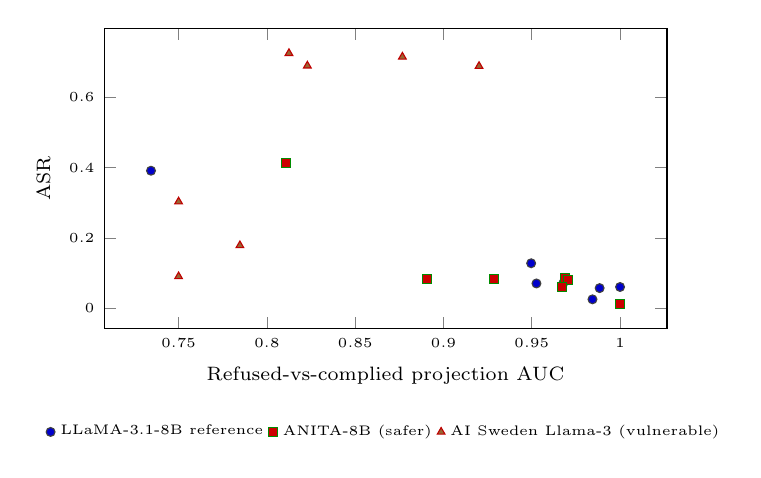
\begin{tikzpicture}
\begin{axis}[width=0.72\linewidth,height=5.4cm,
xlabel={Refused-vs-complied projection AUC},ylabel={ASR},
label style={font=\scriptsize},tick label style={font=\tiny},
legend style={font=\tiny,at={(0.5,-0.28)},anchor=north,draw=none,fill=none,legend columns=3}]
\addplot+[only marks,mark=*,mark size=1.6pt,black!75!white] coordinates {(0.9496527777777778,0.1282051282051282) (0.984375,0.025559105431309903) (1.0,0.06070287539936102) (0.9526515151515151,0.0707395498392283) (0.9884259259259259,0.05750798722044728) (0.734375,0.39158576051779936) (0.9678030303030303,0.07096774193548387)};
\addlegendentry{LLaMA-3.1-8B reference}
\addplot+[only marks,mark=square*,mark size=1.6pt,green!55!black] coordinates {(0.96875,0.08653846153846154) (1.0,0.012779552715654952) (0.9288194444444444,0.08306709265175719) (0.9704861111111112,0.08038585209003216) (0.890625,0.08306709265175719) (0.8107638888888888,0.41423948220064727) (0.9671052631578947,0.06129032258064516)};
\addlegendentry{ANITA-8B (safer)}
\addplot+[only marks,mark=triangle*,mark size=1.6pt,red!75!black] coordinates {(0.9201388888888888,0.6891025641025641) (0.8767361111111112,0.7156549520766773) (0.7847222222222222,0.17891373801916932) (0.8229166666666666,0.6903225806451613) (0.75,0.3035143769968051) (0.75,0.09061488673139159) (0.8125,0.7258064516129032)};
\addlegendentry{AI Sweden Llama-3 (vulnerable)}
\end{axis}
\end{tikzpicture}
\caption[Refusal-signal separability versus ASR]{In-sample refusal-signal separability versus behavioural ASR across 21 model--language cells. The pooled association is negative, but the within-model direction is heterogeneous; Spearman coefficients are reported in the text.}
\label{fig:mechanistic-separability-vs-asr}
\fonte{Author.}
\end{figure}
}

\newcommand{\MechLayerSweepFigure}{%
\begin{figure}[htbp]
\centering
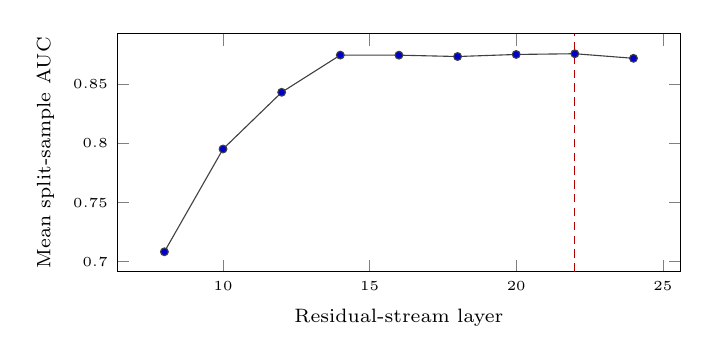
\begin{tikzpicture}
\begin{axis}[width=0.72\linewidth,height=4.6cm,
xlabel={Residual-stream layer},ylabel={Mean split-sample AUC},
label style={font=\scriptsize},tick label style={font=\tiny}]
\addplot+[mark=*,mark size=1.4pt,black!75!white] coordinates {(8,0.7083884479717814) (10,0.7952374790495909) (12,0.8431731790945042) (14,0.8745912616254232) (16,0.8745210846013124) (18,0.8733831898298773) (20,0.8751263186433994) (22,0.8757466150711491) (24,0.871869077743819)};
\draw[densely dashed,red!70!black] (axis cs:22,\pgfkeysvalueof{/pgfplots/ymin}) -- (axis cs:22,\pgfkeysvalueof{/pgfplots/ymax});
\end{axis}
\end{tikzpicture}
\caption[Layer sweep for the refusal-outcome direction]{Layer sweep: mean split-sample refused-versus-complied AUC across the three models. The dashed line marks the layer selected using these same test splits, so the peak is a selection criterion rather than an independent performance estimate.}
\label{fig:mechanistic-layer-sweep}
\fonte{Author.}
\end{figure}
}

\newcommand{\MechRefusalProjectionsTable}{%
\begin{table}[htbp]
\centering
\scriptsize
\caption[Refusal-outcome direction diagnostics per model--language cell]{Refusal-outcome direction diagnostics per model--language cell: in-sample within-language projection AUC, mean cross-lingual transfer AUC into the cell, cosine to the aligned-language direction, and frozen behavioural ASR.}
\label{tab:mechanistic-refusal-projections}
\begin{tabular}{llrrrr}
\toprule
Model & Lang. & AUC & Transfer-in & Cosine & ASR \\
\midrule
\texttt{LLaMA-3.1-8B reference} & \texttt{eng} & 0.98 & 0.98 & 1.00 & 2.6\% \\
 & \texttt{ita} & 1.00 & 1.00 & 0.68 & 6.1\% \\
 & \texttt{spa} & 0.99 & 0.98 & 0.69 & 5.8\% \\
 & \texttt{dan} & 0.95 & 0.95 & 0.69 & 12.8\% \\
 & \texttt{nor} & 0.95 & 0.95 & 0.70 & 7.1\% \\
 & \texttt{swe} & 0.97 & 0.96 & 0.74 & 7.1\% \\
 & \texttt{swa} & 0.73 & 0.74 & 0.51 & 39.2\% \\
\midrule
\texttt{ANITA-8B (safer)} & \texttt{eng} & 1.00 & 1.00 & 0.73 & 1.3\% \\
 & \texttt{ita} & 0.93 & 0.93 & 1.00 & 8.3\% \\
 & \texttt{spa} & 0.89 & 0.88 & 0.90 & 8.3\% \\
 & \texttt{dan} & 0.97 & 0.96 & 0.84 & 8.7\% \\
 & \texttt{nor} & 0.97 & 0.96 & 0.84 & 8.0\% \\
 & \texttt{swe} & 0.97 & 0.97 & 0.85 & 6.1\% \\
 & \texttt{swa} & 0.81 & 0.81 & 0.69 & 41.4\% \\
\midrule
\texttt{AI Sweden Llama-3 (vulnerable)} & \texttt{eng} & 0.88 & 0.74 & 0.69 & 71.6\% \\
 & \texttt{ita} & 0.78 & 0.62 & -0.10 & 17.9\% \\
 & \texttt{spa} & 0.75 & 0.63 & 0.11 & 30.4\% \\
 & \texttt{dan} & 0.92 & 0.84 & 0.53 & 68.9\% \\
 & \texttt{nor} & 0.82 & 0.72 & 0.44 & 69.0\% \\
 & \texttt{swe} & 0.81 & 0.67 & 1.00 & 72.6\% \\
 & \texttt{swa} & 0.75 & 0.63 & 0.08 & 9.1\% \\
\bottomrule
\end{tabular}
\fonte{Author.}
\end{table}
}

\newcommand{\MechLanguageDirectionSimilarityTable}{%
\begin{table}[htbp]
\centering
\scriptsize
\caption[Cross-lingual refusal-direction cosine similarity]{Cosine similarity of each attack language's refusal-outcome direction to the model's aligned-language direction and to the model's pooled direction.}
\label{tab:mechanistic-language-direction-similarity}
\begin{tabular}{llrr}
\toprule
Model & Lang. & Cos.\ aligned & Cos.\ pooled \\
\midrule
\texttt{LLaMA-3.1-8B reference} & \texttt{eng} & 1.00 & 0.80 \\
 & \texttt{ita} & 0.68 & 0.92 \\
 & \texttt{spa} & 0.69 & 0.93 \\
 & \texttt{dan} & 0.69 & 0.95 \\
 & \texttt{nor} & 0.70 & 0.94 \\
 & \texttt{swe} & 0.74 & 0.96 \\
 & \texttt{swa} & 0.51 & 0.77 \\
\midrule
\texttt{ANITA-8B (safer)} & \texttt{eng} & 0.73 & 0.81 \\
 & \texttt{ita} & 1.00 & 0.90 \\
 & \texttt{spa} & 0.90 & 0.92 \\
 & \texttt{dan} & 0.84 & 0.96 \\
 & \texttt{nor} & 0.84 & 0.96 \\
 & \texttt{swe} & 0.85 & 0.96 \\
 & \texttt{swa} & 0.69 & 0.79 \\
\midrule
\texttt{AI Sweden Llama-3 (vulnerable)} & \texttt{eng} & 0.69 & 0.76 \\
 & \texttt{ita} & -0.10 & 0.49 \\
 & \texttt{spa} & 0.11 & 0.57 \\
 & \texttt{dan} & 0.53 & 0.87 \\
 & \texttt{nor} & 0.44 & 0.77 \\
 & \texttt{swe} & 1.00 & 0.63 \\
 & \texttt{swa} & 0.08 & 0.44 \\
\bottomrule
\end{tabular}
\fonte{Author.}
\end{table}
}

\newcommand{\MechInterventionTable}{%
\begin{table}[htbp]
\centering
\scriptsize
\caption[Addition-only refusal-strengthening intervention outcomes]{Addition-only intervention on previously unsafe prompts from the direction-estimation sample. Explicit refusal requires agreement between the StrongREJECT label and fixed marker matching on the backtranslated output. Manual inspection found substantial degeneration at high $\alpha$; still-unsafe uses the StrongREJECT score alone and zero can therefore include refusal, irrelevant output, or degeneration. Other means non-refusal zero-score output; Failed is a count, and the remaining outcome columns are percentages.}
\label{tab:mechanistic-intervention}
\setlength{\tabcolsep}{3pt}\begin{tabular}{lrrrrrrr}
\toprule
Model & $\alpha$ & $n$ & Explicit & Judge-only & Unsafe & Other & Failed \\
\midrule
\texttt{LLaMA-3.1-8B reference} & 0.5 & 137 & 70.1\% & 13.1\% & 13.1\% & 3.6\% & 0 \\
 & 1 & 137 & 85.4\% & 10.2\% & 1.5\% & 2.9\% & 0 \\
 & 2 & 137 & 0.0\% & 89.8\% & 0.0\% & 10.2\% & 0 \\
\midrule
\texttt{ANITA-8B (safer)} & 0.5 & 143 & 73.4\% & 9.1\% & 16.8\% & 0.7\% & 0 \\
 & 1 & 143 & 97.9\% & 0.7\% & 0.0\% & 1.4\% & 0 \\
 & 2 & 143 & 45.5\% & 51.7\% & 0.0\% & 2.8\% & 0 \\
\midrule
\texttt{AI Sweden Llama-3 (vulnerable)} & 0.5 & 168 & 16.1\% & 39.3\% & 36.3\% & 8.3\% & 0 \\
 & 1 & 168 & 11.3\% & 83.9\% & 0.0\% & 4.8\% & 0 \\
 & 2 & 168 & 0.0\% & 95.2\% & 0.0\% & 4.8\% & 0 \\
\bottomrule
\end{tabular}
\fonte{Author.}
\end{table}
}
